\documentclass[11pt]{article}

% For notes stored at notes/<domain>/<slug>/note.tex.
% Shared preamble for youtube_notes educational LaTeX notes.
% Intended for LuaLaTeX.

\usepackage[a4paper,margin=1in]{geometry}
\usepackage{fontspec}
\usepackage{microtype}
\usepackage{amsmath}
\usepackage{amssymb}
\usepackage{amsthm}
\usepackage{mathtools}
\usepackage{graphicx}
\usepackage{booktabs}
\usepackage{array}
\usepackage{xcolor}
\usepackage{enumitem}
\usepackage{tcolorbox}
\usepackage{tikz}
\usepackage{pgfplots}
\usepackage{siunitx}
\usepackage{hyperref}
\usepackage[nameinlink,noabbrev]{cleveref}

\pgfplotsset{compat=1.18}
\tcbuselibrary{breakable,skins}

\setmainfont{Latin Modern Roman}
\setsansfont{Latin Modern Sans}
\setmonofont{Latin Modern Mono}

\definecolor{ynBlue}{HTML}{1F4E79}
\definecolor{ynTeal}{HTML}{1B7F79}
\definecolor{ynGreen}{HTML}{2F7D32}
\definecolor{ynAmber}{HTML}{B86E00}
\definecolor{ynRed}{HTML}{A83232}
\definecolor{ynGray}{HTML}{F4F6F8}
\definecolor{ynInk}{HTML}{1F2933}

\hypersetup{
  colorlinks=true,
  linkcolor=ynBlue,
  citecolor=ynTeal,
  urlcolor=ynBlue,
  pdftitle={YouTube Note},
  pdfauthor={youtube_notes}
}

\setlist[itemize]{leftmargin=*,itemsep=0.2em,topsep=0.3em}
\setlist[enumerate]{leftmargin=*,itemsep=0.2em,topsep=0.3em}
\setlength{\parindent}{0pt}
\setlength{\parskip}{0.65em}

\numberwithin{equation}{section}

\theoremstyle{plain}
\newtheorem{theorem}{Theorem}[section]
\newtheorem{lemma}[theorem]{Lemma}
\newtheorem{proposition}[theorem]{Proposition}
\newtheorem{corollary}[theorem]{Corollary}

\theoremstyle{definition}
\newtheorem{definition}{Definition}[section]
\newtheorem{example}{Example}[section]

\theoremstyle{remark}
\newtheorem*{remark}{Remark}


% Common mathematical macros for generated notes.

\newcommand{\R}{\mathbb{R}}
\newcommand{\N}{\mathbb{N}}
\newcommand{\Z}{\mathbb{Z}}
\newcommand{\Q}{\mathbb{Q}}
\newcommand{\C}{\mathbb{C}}

\newcommand{\E}{\mathbb{E}}
\newcommand{\Var}{\operatorname{Var}}
\newcommand{\Cov}{\operatorname{Cov}}
\newcommand{\Corr}{\operatorname{Corr}}
\newcommand{\Prob}{\mathbb{P}}

\newcommand{\dd}{\,\mathrm{d}}
\newcommand{\grad}{\nabla}
\newcommand{\argmin}{\operatorname*{arg\,min}}
\newcommand{\argmax}{\operatorname*{arg\,max}}
\newcommand{\diag}{\operatorname{diag}}
\newcommand{\rank}{\operatorname{rank}}
\newcommand{\tr}{\operatorname{tr}}
\newcommand{\spanof}{\operatorname{span}}

\newcommand{\abs}[1]{\left\lvert #1 \right\rvert}
\newcommand{\norm}[1]{\left\lVert #1 \right\rVert}
\newcommand{\inner}[2]{\left\langle #1, #2 \right\rangle}
\newcommand{\set}[1]{\left\{ #1 \right\}}
\newcommand{\paren}[1]{\left( #1 \right)}
\newcommand{\bracket}[1]{\left[ #1 \right]}
\newcommand{\given}{\,\middle|\,}

\newcommand{\vecx}{\mathbf{x}}
\newcommand{\vecy}{\mathbf{y}}
\newcommand{\vectheta}{\boldsymbol{\theta}}


% Boxed educational environments for generated notes.

\newtcolorbox{definitionbox}[1][]{
  enhanced,
  breakable,
  colback=ynBlue!4,
  colframe=ynBlue,
  coltitle=white,
  fonttitle=\bfseries,
  title=Definition,
  sharp corners,
  boxrule=0.8pt,
  left=8pt,
  right=8pt,
  top=7pt,
  bottom=7pt,
  #1
}

\newtcolorbox{intuitionbox}[1][]{
  enhanced,
  breakable,
  colback=ynTeal!5,
  colframe=ynTeal,
  coltitle=white,
  fonttitle=\bfseries,
  title=Intuition,
  sharp corners,
  boxrule=0.8pt,
  left=8pt,
  right=8pt,
  top=7pt,
  bottom=7pt,
  #1
}

\newtcolorbox{warningbox}[1][]{
  enhanced,
  breakable,
  colback=ynAmber!8,
  colframe=ynAmber,
  coltitle=white,
  fonttitle=\bfseries,
  title=Warning,
  sharp corners,
  boxrule=0.8pt,
  left=8pt,
  right=8pt,
  top=7pt,
  bottom=7pt,
  #1
}

\newtcolorbox{examplebox}[1][]{
  enhanced,
  breakable,
  colback=ynGreen!5,
  colframe=ynGreen,
  coltitle=white,
  fonttitle=\bfseries,
  title=Worked Example,
  sharp corners,
  boxrule=0.8pt,
  left=8pt,
  right=8pt,
  top=7pt,
  bottom=7pt,
  #1
}

\newtcolorbox{resultbox}[1][]{
  enhanced,
  breakable,
  colback=ynRed!4,
  colframe=ynRed,
  coltitle=white,
  fonttitle=\bfseries,
  title=Key Result,
  sharp corners,
  boxrule=0.8pt,
  left=8pt,
  right=8pt,
  top=7pt,
  bottom=7pt,
  #1
}

\newtcolorbox{checkpointbox}[1][]{
  enhanced,
  breakable,
  colback=ynGray,
  colframe=ynInk,
  coltitle=white,
  fonttitle=\bfseries,
  title=Checkpoint,
  sharp corners,
  boxrule=0.8pt,
  left=8pt,
  right=8pt,
  top=7pt,
  bottom=7pt,
  #1
}



\DeclareMathOperator{\conv}{conv}
\DeclareMathOperator{\Foci}{Foci}
\newcommand{\ii}{\mathrm{i}}
\hypersetup{
  pdftitle={Marden's Theorem: Cubic Critical Points and Ellipse Foci},
  pdfauthor={youtube notes}
}

\title{Marden's Theorem\\\large Cubic Critical Points and Ellipse Foci}
\author{youtube\_notes}
\date{2026-05-06}

\begin{document}

\maketitle

\begin{abstract}
Marden's theorem says that a purely algebraic operation and a purely geometric construction secretly produce the same two points. Start with a cubic polynomial whose three complex roots are non-collinear, so that they form a triangle in the complex plane. The derivative is a quadratic, so it has two roots. The theorem states that those two derivative roots are exactly the foci of the Steiner inellipse: the unique ellipse inscribed in the triangle and tangent to the three sides at their midpoints. This note develops the theorem from the first algebraic clue, works through a concrete cubic, gives a proof based on Carlson's normalization argument, and closes with the electrostatic interpretation coming from the logarithmic derivative.
\end{abstract}

\tableofcontents
\newpage

\section{The Question}

Let
\begin{align}
  p(z)=(z-a)(z-b)(z-c),
  \qquad a,b,c\in \C,
  \label{eq:cubic-from-roots}
\end{align}
where the three roots are distinct and non-collinear. We identify a complex number \(x+\ii y\) with the point \((x,y)\) in the plane, so the roots \(a,b,c\) form a triangle.

The derivative \(p'(z)\) is quadratic. Therefore it has two roots, counted with multiplicity. Call them \(f_1\) and \(f_2\):
\begin{align}
  p'(f_1)=p'(f_2)=0.
\end{align}

The Gauss--Lucas theorem already gives a first location result: the roots of \(p'\) lie in the convex hull of the roots of \(p\). In this cubic case, that means \(f_1\) and \(f_2\) lie inside or on the triangle \(\triangle abc\). But Gauss--Lucas does not say where inside the triangle they are.

\begin{intuitionbox}
The puzzle is that a cubic gives three points, while its derivative gives two points. Ordinary triangle centers usually come one at a time. Marden's theorem says the correct pair is not arbitrary: it is the pair of foci of a very special ellipse attached to the same triangle.
\end{intuitionbox}

\section{The Steiner Inellipse}

\begin{definitionbox}[title=Steiner inellipse]
For a non-degenerate triangle, the \emph{Steiner inellipse} is the unique ellipse inscribed in the triangle and tangent to each side at that side's midpoint.
\end{definitionbox}

For the triangle with complex vertices \(a,b,c\), the side midpoints are
\begin{align}
  m_{ab}=\frac{a+b}{2},
  \qquad
  m_{bc}=\frac{b+c}{2},
  \qquad
  m_{ca}=\frac{c+a}{2}.
\end{align}
The center of the Steiner inellipse is the centroid
\begin{align}
  G=\frac{a+b+c}{3}.
  \label{eq:centroid}
\end{align}

There is a quick way to remember why the centroid appears. Start with an equilateral triangle: its Steiner inellipse is just the incircle, and its center is the centroid. Every triangle is an affine image of an equilateral triangle, and affine maps preserve midpoints, tangencies, and barycenters. Hence the midpoint-tangent ellipse of the image triangle is centered at the image of the original centroid.

\begin{warningbox}[title=Affine warning]
The previous paragraph is safe for centers, midpoints, tangencies, and ellipses. It is not, by itself, a proof about foci. Foci are metric objects: they are defined using Euclidean distance. A general affine map can shear or stretch distances differently in different directions, so it does not generally send the foci of one ellipse to the foci of the image ellipse.
\end{warningbox}

\section{The Theorem}

\begin{theorem}[Marden's theorem]
\label{thm:marden}
Let \(p(z)\) be a cubic polynomial whose three roots \(a,b,c\) are distinct and non-collinear points in the complex plane. Let \(E\) be the Steiner inellipse of the triangle \(\triangle abc\). Then
\begin{align}
  \Foci(E)=\set{z\in\C:p'(z)=0}.
\end{align}
In other words, the two roots of the derivative are exactly the two foci of the Steiner inellipse.
\end{theorem}

The result is often called Marden's theorem, although the nineteenth-century result is due to J\"org Siebeck. Dan Kalman's modern exposition helped make it widely known in elementary form.

\section{The First Algebraic Clue}

Write the elementary symmetric sums as
\begin{align}
  s_1=a+b+c,\qquad
  s_2=ab+bc+ca,\qquad
  s_3=abc.
\end{align}
Then
\begin{align}
  p(z)
    &=z^3-s_1z^2+s_2z-s_3, \\
  p'(z)
    &=3z^2-2s_1z+s_2.
  \label{eq:cubic-derivative}
\end{align}

Solving \(p'(z)=0\) gives an explicit formula for the two critical points:
\begin{align}
  0&=3z^2-2s_1z+s_2,\\
  z
    &=\frac{2s_1\pm \sqrt{4s_1^2-12s_2}}{6} \\
    &=\frac{s_1\pm \sqrt{s_1^2-3s_2}}{3}.
  \label{eq:critical-point-formula}
\end{align}
Thus
\begin{align}
  f_{1,2}
  =
  \frac{a+b+c\pm \sqrt{(a+b+c)^2-3(ab+bc+ca)}}{3}.
\end{align}

Now apply Vieta's formula to the quadratic \(p'(z)\). Since the sum of the roots of \(Az^2+Bz+C\) is \(-B/A\),
\begin{align}
  f_1+f_2
    &=\frac{2s_1}{3},\\
  \frac{f_1+f_2}{2}
    &=\frac{s_1}{3}
      =\frac{a+b+c}{3}
      =G.
  \label{eq:critical-points-midpoint}
\end{align}

\begin{resultbox}
The midpoint of the two derivative roots is the centroid of the triangle. This does not prove Marden's theorem, but it shows that the derivative roots already know about a central geometric feature of the triangle.
\end{resultbox}

This is exactly what we should expect if Marden's theorem is true. The midpoint of the two foci of any ellipse is the center of the ellipse, and the center of the Steiner inellipse is \(G\).

\section{A Worked Cubic}

Consider the cubic from the source video:
\begin{align}
  p(z)=(z-1)(z-\ii)(z-2).
\end{align}
Here
\begin{align}
  a=1,\qquad b=\ii,\qquad c=2,
\end{align}
so
\begin{align}
  s_1&=3+\ii,\\
  s_2&=1\cdot \ii+\ii\cdot 2+2\cdot 1=2+3\ii,\\
  s_3&=1\cdot \ii\cdot 2=2\ii.
\end{align}
Therefore
\begin{align}
  p(z)
    &=z^3-(3+\ii)z^2+(2+3\ii)z-2\ii,\\
  p'(z)
    &=3z^2-2(3+\ii)z+(2+3\ii).
\end{align}

The discriminant term in \cref{eq:critical-point-formula} is
\begin{align}
  s_1^2-3s_2
    &=(3+\ii)^2-3(2+3\ii)\\
    &=(8+6\ii)-(6+9\ii)\\
    &=2-3\ii.
\end{align}
Hence the two derivative roots are
\begin{align}
  f_{1,2}=\frac{3+\ii\pm\sqrt{2-3\ii}}{3}.
  \label{eq:example-critical-points}
\end{align}
Numerically,
\begin{align}
  f_1&\approx 1.55805+0.03467\ii,\\
  f_2&\approx 0.44195+0.63199\ii.
\end{align}
Their midpoint is
\begin{align}
  \frac{f_1+f_2}{2}=1+\frac{1}{3}\ii,
\end{align}
which is exactly the centroid of the triangle with vertices \(1,\ii,2\).

\begin{figure}[htbp]
  \centering
  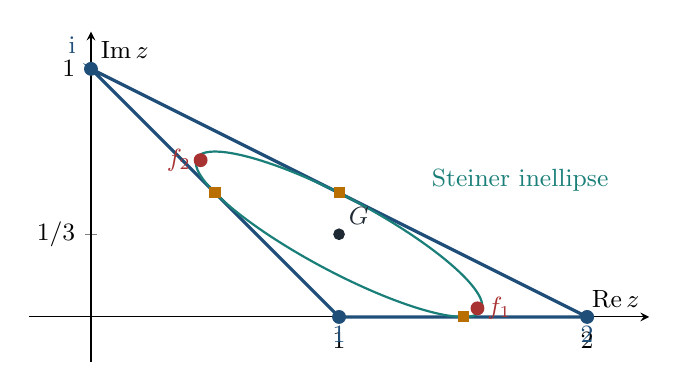
\begin{tikzpicture}
    \begin{axis}[
      axis equal image,
      width=0.78\linewidth,
      xmin=-0.25,xmax=2.25,
      ymin=-0.18,ymax=1.15,
      axis lines=middle,
      xlabel={\(\operatorname{Re} z\)},
      ylabel={\(\operatorname{Im} z\)},
      xtick={0,1,2},
      ytick={0,0.333333,1},
      yticklabels={\(0\),\(1/3\),\(1\)},
      tick label style={font=\small},
      label style={font=\small},
      clip=false
    ]
      \addplot[very thick, ynBlue] coordinates {(1,0) (0,1) (2,0) (1,0)};
      \addplot[
        domain=0:360,
        samples=220,
        smooth,
        thick,
        ynTeal
      ]
      ({1 + 0.6500236*cos(x)*0.8816746 - 0.1480332*sin(x)*(-0.4718579)},
       {0.3333333 + 0.6500236*cos(x)*(-0.4718579) + 0.1480332*sin(x)*0.8816746});
      \addplot[only marks, mark=*, mark size=2.3pt, ynBlue]
        coordinates {(1,0) (0,1) (2,0)};
      \addplot[only marks, mark=*, mark size=2.3pt, ynRed]
        coordinates {(1.55805,0.03467) (0.44195,0.63199)};
      \addplot[only marks, mark=*, mark size=1.9pt, ynInk]
        coordinates {(1,0.333333)};
      \addplot[only marks, mark=square*, mark size=1.8pt, ynAmber]
        coordinates {(0.5,0.5) (1,0.5) (1.5,0)};

      \node[font=\small, ynBlue, below] at (axis cs:1,0) {\(1\)};
      \node[font=\small, ynBlue, above left, xshift=-2pt, yshift=2pt] at (axis cs:0,1) {\(\ii\)};
      \node[font=\small, ynBlue, below] at (axis cs:2,0) {\(2\)};
      \node[font=\small, ynRed, right] at (axis cs:1.55805,0.03467) {\(f_1\)};
      \node[font=\small, ynRed, left] at (axis cs:0.44195,0.63199) {\(f_2\)};
      \node[font=\small, ynInk, above right] at (axis cs:1,0.333333) {\(G\)};
      \node[font=\small, ynTeal] at (axis cs:1.73,0.55) {Steiner inellipse};
    \end{axis}
  \end{tikzpicture}
  \caption{For \(p(z)=(z-1)(z-\ii)(z-2)\), the two roots of \(p'\) lie at the foci of the Steiner inellipse. The amber squares mark the side midpoints where the ellipse is tangent to the triangle.}
  \label{fig:example-steiner-inellipse}
\end{figure}

\begin{checkpointbox}
The decimal values in \cref{fig:example-steiner-inellipse} are not independent evidence for the theorem; they are a consistency check. The exact statement is \cref{eq:example-critical-points}, and Marden's theorem explains why those same exact points are the foci of the ellipse.
\end{checkpointbox}

\section{Proof of Marden's Theorem}

The tempting one-sentence proof is: prove the equilateral case, then use affine transformations. That slogan hides a problem: affine transformations do not preserve foci in general. The proof below uses an affine stretch more carefully. We first place the actual foci where we want them, then use the stretch only to extract algebraic information about the original roots.

\begin{proof}[Proof of \cref{thm:marden}]
Let \(E\) be the Steiner inellipse of \(\triangle abc\). By translating, rotating, and uniformly scaling the complex plane, we may assume that the center of \(E\) is \(0\) and that its two foci are \(\pm c\) on the real axis, with \(c\ge 0\). These transformations are complex similarities, so they preserve foci. They also transform derivative roots correctly: if \(T(w)=\alpha w+\beta\) with \(\alpha\ne0\) and \(q(w)=p(T(w))\), then
\begin{align}
  q'(w)=\alpha p'(T(w)).
\end{align}
Thus \(q'(w)=0\) exactly when \(p'(T(w))=0\).

Let the semimajor and semiminor axes of \(E\) have lengths \(A\) and \(B\), with the major axis on the real axis. Then
\begin{align}
  c^2=A^2-B^2,
  \label{eq:focal-length}
\end{align}
and the ellipse has equation
\begin{align}
  \frac{x^2}{A^2}+\frac{y^2}{B^2}=1.
\end{align}
Write the three roots as
\begin{align}
  z_j=x_j+\ii y_j,\qquad j=0,1,2,
\end{align}
and use the cyclic convention \(z_3=z_0\).

Now apply the horizontal stretch
\begin{align}
  x+\ii y\longmapsto \zeta=\frac{B}{A}x+\ii y.
  \label{eq:horizontal-stretch}
\end{align}
This sends \(E\) to the circle of radius \(B\), because
\begin{align}
  X=\frac{B}{A}x,\qquad Y=y
  \quad\Longrightarrow\quad
  X^2+Y^2=B^2.
\end{align}
It also sends the triangle to a new triangle whose incircle is tangent to the three sides at their midpoints. A triangle with an incircle touching all three sides at their midpoints is equilateral: equal tangent lengths from each vertex force the three side lengths to be equal.

Thus the transformed vertices
\begin{align}
  \zeta_j=\frac{B}{A}x_j+\ii y_j
\end{align}
form an equilateral triangle centered at \(0\), with inradius \(B\). Therefore its circumradius is \(2B\), and
\begin{align}
  \sum_{j=0}^{2}\zeta_j=0,
  \qquad
  \sum_{j=0}^{2}\zeta_j^2=0,
  \qquad
  |\zeta_j|=2B \quad (j=0,1,2).
  \label{eq:equilateral-relations}
\end{align}

From \(\sum \zeta_j=0\), we get
\begin{align}
  \sum_{j=0}^{2}x_j=0,
  \qquad
  \sum_{j=0}^{2}y_j=0,
  \qquad
  \sum_{j=0}^{2}z_j=0.
  \label{eq:sum-z-zero}
\end{align}
With the root sum equal to zero, the cubic has the form
\begin{align}
  p(z)
    &=\prod_{j=0}^{2}(z-z_j)\\
    &=z^3+\left(\sum_{j=0}^{2}z_jz_{j+1}\right)z-z_0z_1z_2.
  \label{eq:centered-cubic-proof}
\end{align}
So
\begin{align}
  p'(z)=3z^2+\sum_{j=0}^{2}z_jz_{j+1}.
  \label{eq:derivative-proof-form}
\end{align}
To prove that \(p'(z)\) has roots \(\pm c\), it is enough to show
\begin{align}
  \sum_{j=0}^{2}z_jz_{j+1}=-3c^2.
  \label{eq:target-cyclic-sum}
\end{align}

Because \(\sum z_j=0\), squaring gives
\begin{align}
  0
    &=\left(\sum_{j=0}^{2}z_j\right)^2\\
    &=\sum_{j=0}^{2}z_j^2
      +2\sum_{j=0}^{2}z_jz_{j+1}.
  \label{eq:square-sum-zero}
\end{align}
Thus \cref{eq:target-cyclic-sum} will follow once we prove
\begin{align}
  \sum_{j=0}^{2}z_j^2=6c^2.
  \label{eq:sum-squares-target}
\end{align}

Let \(\lambda=B/A\), and put
\begin{align}
  X_2=\sum_{j=0}^{2}x_j^2,\qquad
  Y_2=\sum_{j=0}^{2}y_j^2.
\end{align}
The relation \(\sum \zeta_j^2=0\) says
\begin{align}
  0
    &=\sum_{j=0}^{2}\left(\lambda x_j+\ii y_j\right)^2\\
    &=\lambda^2X_2-Y_2
      +2\ii\lambda\sum_{j=0}^{2}x_jy_j.
\end{align}
Hence
\begin{align}
  \sum_{j=0}^{2}x_jy_j=0,
  \qquad
  \lambda^2X_2=Y_2.
  \label{eq:lambda-relations}
\end{align}
The relation \(|\zeta_j|=2B\) for all three vertices gives
\begin{align}
  \sum_{j=0}^{2}|\zeta_j|^2
    &=3(2B)^2,\\
  \lambda^2X_2+Y_2
    &=12B^2.
  \label{eq:norm-relation}
\end{align}
Combining \cref{eq:lambda-relations,eq:norm-relation},
\begin{align}
  X_2=6A^2,
  \qquad
  Y_2=6B^2.
\end{align}
Therefore
\begin{align}
  \sum_{j=0}^{2}z_j^2
    &=\sum_{j=0}^{2}(x_j+\ii y_j)^2\\
    &=X_2-Y_2+2\ii\sum_{j=0}^{2}x_jy_j\\
    &=6A^2-6B^2\\
    &=6c^2,
\end{align}
using \cref{eq:focal-length}. This proves \cref{eq:sum-squares-target}. Then \cref{eq:square-sum-zero} gives
\begin{align}
  \sum_{j=0}^{2}z_jz_{j+1}=-3c^2.
\end{align}
Finally,
\begin{align}
  p'(z)=3z^2-3c^2=3(z-c)(z+c).
\end{align}
The roots of \(p'\) are exactly \(c\) and \(-c\), which are the foci of \(E\). Undoing the initial similarity transformation proves the theorem in the original coordinates.
\end{proof}

\begin{checkpointbox}
The equilateral case is contained in the proof. If \(A=B\), then \(c=0\), the Steiner inellipse is a circle, and the derivative has a double root at the centroid.
\end{checkpointbox}

\section{The Electrostatic Interpretation}

There is another way to read the equation \(p'(z)=0\). For
\begin{align}
  p(z)=\prod_{r\in\{a,b,c\}}(z-r),
\end{align}
the logarithmic derivative is
\begin{align}
  \frac{p'(z)}{p(z)}
    =
    \frac{1}{z-a}+\frac{1}{z-b}+\frac{1}{z-c},
  \qquad z\notin\{a,b,c\}.
  \label{eq:logarithmic-derivative}
\end{align}
Away from the roots, \(p(z)\ne 0\), so
\begin{align}
  p'(z)=0
  \quad\Longleftrightarrow\quad
  \frac{1}{z-a}+\frac{1}{z-b}+\frac{1}{z-c}=0.
  \label{eq:field-cancellation}
\end{align}

This is the algebraic form of a balance condition. In a two-dimensional logarithmic potential, the field contribution from a source at \(r\) points along \(z-r\) and has magnitude proportional to \(1/|z-r|\). Up to complex conjugation, this contribution is represented by
\begin{align}
  \frac{z-r}{|z-r|^2}=\frac{1}{\overline{z-r}}.
\end{align}
Thus \cref{eq:field-cancellation} says that the three equal contributions cancel. The two critical points of the cubic are equilibrium points of this logarithmic field.

\begin{intuitionbox}
Marden's theorem lets the same two points wear three different names: roots of the derivative, foci of the Steiner inellipse, and equilibrium points for the logarithmic field generated by the three roots.
\end{intuitionbox}

\section{Scope and Special Cases}

\begin{itemize}
  \item \textbf{Non-collinear distinct roots.} This is the standard setting of Marden's theorem: the roots form a genuine triangle and the Steiner inellipse is non-degenerate.
  \item \textbf{Equilateral triangle.} The Steiner inellipse is the incircle, so its foci coincide at the center. Algebraically, the derivative has a double root at the centroid.
  \item \textbf{Collinear or repeated roots.} The triangle degenerates. One can discuss limiting versions, but the clean geometric statement needs modification.
  \item \textbf{Higher-degree polynomials.} Gauss--Lucas still places the roots of \(p'\) in the convex hull of the roots of \(p\), but the simple triangle-and-Steiner-inellipse picture is special to the cubic setting.
\end{itemize}

\section{Exercises}

\begin{enumerate}
  \item Let \(p(z)=z^3-1\). Compute the roots of \(p\), the roots of \(p'\), and explain the corresponding Steiner inellipse.

  \item Let \(p(z)=z(z-1)(z-\ii)\). Compute \(p'(z)\), solve \(p'(z)=0\), and verify that the average of the two derivative roots is the centroid of the triangle with vertices \(0,1,\ii\).

  \item Prove that if an incircle touches all three sides of a triangle at their midpoints, then the triangle is equilateral.

  \item A unit circle centered at the origin has both foci at \(0\). Apply the affine stretch \((x,y)\mapsto (2x,y)\). What are the foci of the image ellipse? Use this to explain why arbitrary affine maps do not preserve foci.
\end{enumerate}

\section*{References and Source Note}
\addcontentsline{toc}{section}{References and Source Note}

This note is based primarily on the blueprint generated from the video \emph{The Biggest Coincidence In Math: Marden's Theorem} by Quantia. The proof style follows the standard Carlson/Kalman normalization argument rather than the shorter affine slogan, because the latter can obscure the role of foci.

\begin{itemize}
  \item Dan Kalman, ``An Elementary Proof of Marden's Theorem,'' \emph{The American Mathematical Monthly}, 115(4), 330--338, 2008. DOI: \url{https://doi.org/10.1080/00029890.2008.11920532}.
  \item J\"org Siebeck, ``\"Uber eine neue analytische Behandlungweise der Brennpunkte,'' \emph{Journal f\"ur die reine und angewandte Mathematik}, 64, 175--182, 1864.
  \item Morris Marden, \emph{Geometry of Polynomials}, Mathematical Surveys, vol. 3, American Mathematical Society.
\end{itemize}

\end{document}
